%!TEX root = root.tex

\chapter{Random Graph Models}
\label{chap:random_graphs}
%\chaptermark{Second Chapter Heading}

Our main focus of this work is a collection of random graphs. As a first step, we will introduce some models for a single random graph in this chapter. These important components will not only lead to our model for a collection of graphs but also motivate our estimators later in Chapter~\ref{chap:llg} and Chapter~\ref{chap:robust_llg}.

We start the chapter with some basic concepts of graphs and random graphs in Section~\ref{sec:graphs_random_graphs}. Then in Section~\ref{sec:unweighted_graphs}, random graph models for unweighted graphs are introduced. In particular, it is concerned with independent edge model, random dot product graph, and stochastic blockmodel. Their relationship will also be discussed. Section~\ref{sec:weighted_graphs} generalizes all three models introduced in Section~\ref{sec:unweighted_graphs} so that they can be adapted to weighted graphs.


\section{Graphs and Random Graphs}
\label{sec:graphs_random_graphs}

In this section we will introduce some basic concepts of graphs and random graphs. 

\subsection{Basic Concepts of Graphs}
\label{sec:graph_concept}

A {\em{graph}} is an ordered pair $G = (V, E)$ comprising a set $V$ of vertices together with a set $E$ of edges. Denote the number of vertices $|V|$ to be $n$. Without loss of generality, we assume $V = [n] = \{1, 2, \dots, n\}$. Each edge is associated with two vertices. We say a graph has no self-loops if each edge is associated with two distinct vertices. And a graph is undirected if all its edges have no orientation. Thus for a undirected graph without self-loops, we have the edge set $E \subset \{ \{u, v\}: u, v \in V, u \ne v \}$. This will be our basic setting throughout the entire paper.

Every graph can be represented in the form of adjacency matrix $a \in \mathcal{A}$. For unweighted graphs, $\mathcal{A} = \{ 0, 1 \}^{n \times n}$ so that the adjacency matrices are binary. For $i, j \in [n]$, $a_{ij} = 1$ indicates that there is an edge from vertex $i$ to vertex $j$ and $a_{ij} = 0$ otherwise. Note that $a$ is always symmetric since we assume the graphs to be undirected in this work. Thus $a_{ij} = 1$ means there is an edge between vertex $i$ and vertex $j$ and $a_{ji} = 1$ as well. For weighted graphs, each edge is assigned with a positive real-valued weight, i.e. $\mathcal{A} = \mathbb{R}^{n \times n}_{\ge 0}$. Similarly, $a_{ij} > 0$ denotes the weight assigned to the edge between vertex $i$ and vertex $j$, and $a_{ij} = 0$ means there is no edge between these two vertices.

As mentioned above, we assume the graph has no self-loops and are undirected. So every adjacency matrix $a$ is hollow and symmetric, that is $a_{ii} = 0$ for $i \in [n]$ and $a_{ij} = a_{ji}$ for $i, j \in [n]$. This is always assumed without specific clarifications in later sections.


\subsection{Random Graphs}
\label{sec:random_graphs}
A random graph is a graph with fixed vertex set whose edges are randomly distributed with respect to some distributions. Mathematically, a random graph $A: \Omega \mapsto \mathcal{A}$ is a map from the probability space $(\Omega, \mathcal{F}, \mathbb{P})$ to the space of all adjacency matrices on $n$ vertices.

\begin{example}[Erd\H{o}s-R{\'e}nyi Graphs]
\label{example:ER}
The first random graph model is the {\em{Erd\H{o}s-R{\'e}nyi graphs} (ER)} introduced by \citep{gilbert1959random}.  They are unweighted graphs where each edge is present with the same probability $p \in [0, 1]$ independently. In our setting (undirected graphs without self-loops), that is $A_{ij} \stackrel{iid}{\sim} \mathrm{Bernoulli}(p)$ for $i, j \in [n]$ with $i < j$. Thus for $a \in \mathcal{A}$ we have
\[
	\mathbb{P}(A = a) = \prod_{i < j} p^{a_{ij}} (1 - p)^{1 - a_{ij}}.
\]
\end{example}

In later sections, we will introduce other random graph models which capture different properties of the graphs in practice respectively.







\section{Unweighted Random Graph Models}
\label{sec:unweighted_graphs}

In this section, we will focus on unweighted graphs and introduce three important models, i.e. independent edge model, random dot product graph, and stochastic blockmodel. 



\subsection{Independent Edge Model}
\label{sec:IEM}

As introduced in Example~\ref{example:ER}, we see ER model is quite restrictive since all edges follow the same Bernoulli distribution with parameter $p$. Here we consider a much more general model.

\begin{definition}[Independent Edge Model]
\label{def:IEM}
Under an {\em{independent edge model} (IEM)} proposed by \citet{bollobas2007phase}, for $i, j \in [n]$ and $i < j$, the edge between vertex $i$ and vertex $j$ is present with probability $p_{ij} \in [0, 1]$ independently, i.e. $A_{ij} \stackrel{ind}{\sim} \mathrm{Bernoulli}(p_{ij})$. Let $P = (p_{ij})_{i,j = 1}^n \in [0, 1]^{n \times n}$ be the parameter matrix consists of all probabilities for Bernoulli distributions, then the model is denoted by IEM(P).
Thus for $a \in \mathcal{A}$ we have
\[
	\mathbb{P}(A = a) = \prod_{i < j} p_{ij}^{a_{ij}} (1 - p_{ij})^{1 - a_{ij}}.
\]
\end{definition}

Note that the graphs considered in this paper are always assumed to be undirected without self-loops, thus the parameter matrix $P$ needs to be symmetric and hollow. However, for convenience, we still define the parameters to be an $n$-by-$n$ matrix while only $n \choose 2$ of them are effective.

Compared to the ER model, IEM allows the probabilities of the existence of the edges to vary while keeping the independence. Different probabilities give IEM the freedom to include a wide range of random graph distributions, but definitely not all of them because of independence assumption. The most general model is a multinomial distribution with $2^{n \choose 2}$ choices from all possible unweighted and undirected graphs with no self-loops on $n$ vertices, which imposes no assumptions on the graph structure. While such model is instructive sometimes, IEM will be the most general model we consider in this paper. 



\subsection{Random Dot Product Graph}
\label{sec:RDPG}
For a graph, the adjacencies between vertices generally depend on unobserved properties of the corresponding vertices. For instance, in a social network setting, people are more likely to be friends if they have shared interests; in a connectomics setting, the two brain regions with similar properties will have similar connectivity patterns compared to other regions of the brain.
The latent positions model (LPM) proposed by \citep{hoff2002latent} captures such structure, where each vertex is associated with a latent position that influences the adjacencies for that vertex. In particular, we are interested in the case that the latent positions are random in this work.

\begin{definition}[Latent Position Model]
\label{def:LPM}
Let the latent position for vertex $i$ be a random variable $X_i: \Omega \mapsto \mathcal{X}$, where $\mathcal{X}$ is the latent space and $i \in [n]$. Let the link function be a symmetric map $\kappa: \mathcal{X}^2 \mapsto [0, 1]$. Then under a {\em{latent position model (LPM)}}, for $i, j \in [n]$ and $i < j$, conditioned on their respective latent positions $X_i$ and $X_j$,
\[
	A_{ij} | (X_i, X_j) \stackrel{ind}{\sim} \mathrm{Bernoulli}(\kappa(X_i, X_j)).
\]
Thus for $a \in \mathcal{A}$ we have
\[
	\mathbb{P}(A = a | X_1, \dots, X_n) = \prod_{i < j} \kappa(X_i, X_j)^{a_{ij}} (1 - \kappa(X_i, X_j))^{1 - a_{ij}}.
\]
Let $X_1, \dots, X_n \stackrel{iid}{\sim} F$ for some distribution $F$ on $\mathcal{X}$, then the model is denoted by $\mathrm{LPM}(\mathcal{X}, F, \kappa)$.
\end{definition}

Among all the LPMs, we are particularly interested in the random dot product graph (RDPG) \citep{young2007random, nickel2008random}.

\begin{definition} [Random Dot Product Graph]
\label{def:RDPG}
Let the latent position for vertex $i$ be a random variable $X_i: \Omega \mapsto \mathcal{X} \subset \mathbb{R}^{d}$, where $i \in [n]$ and $\mathcal{X}$ is the latent space such that $x^{\top} y = \sum_{i = 1}^d x_i y_i \in [0, 1]$ for $x, y \in \mathcal{X}$. Then under a {\em{random dot product graph (RDPG)}}, for $i, j \in [n]$ and $i < j$, conditioned on their respective latent positions $X_i$ and $X_j$,
\[
	A_{ij} | (X_i, X_j) \stackrel{ind}{\sim} \mathrm{Bernoulli}(X_i^{\top} X_j).
\]
Thus for $a \in \mathcal{A}$ we have
\[
	\mathbb{P}(A = a | X_1, \dots, X_n) = \prod_{i < j} (X_i^{\top} X_j)^{a_{ij}} (1 - X_i^{\top} X_j)^{1 - a_{ij}}.
\]
Let $X_1, \dots, X_n \stackrel{iid}{\sim} F$ for some distribution $F$ on $\mathcal{X}$, then the model is denoted by $\mathrm{RDPG}(\mathcal{X}, F)$.
Typically,  we write all latent positions together as $X = [X_1, \dots, X_n]^{\top} \in \mathbb{R}^{n \times d}$, where the $i$-th row $X_i^{\top}$ corresponds to the latent position for vertex $i$.
\end{definition}

From the definition above, we see RDPG is actually a special case of LPM with latent space $\mathcal{X} \subset \mathbb{R}^d$ such that $x^{\top} y \in [0, 1]$ for $x, y \in \mathcal{X}$ and link function $\kappa(x, y) = x^{\top} y$.
If $d$ is much smaller than the number of vertices $n$, which is likely to be the case in practice, RDPG is then a more parsimonious model compared to IEM, requiring only $n \cdot d$ parameters rather than $n \choose 2$.

The direction and magnitude of the latent position, which are determined by properties of the corresponding vertex, are the most important factors in RDPG due to the nature of dot product. Vertices with latent positions pointing in similar directions are more likely to have an edge between them compared to those with different directions. Similarly, the magnitude of the latent positions encodes the vertices' overall tendency to form edges. A larger magnitude potentially leads to more edges incident with the vertex.

Conditioned on the latent positions $X$, the RDPG now can be considered to be an $\mathrm{IEM}(P)$ with $P = X X^{\top}$, i.e. an edge between vertex $i$ and vertex $j$ is present with probability $P_{ij} = X_i^{\top} X_j$.
Note that the probability matrix $p$ is the outer product of the latent position matrix $X$ with itself. This imposes two important properties on $P$ under RDPG, namely that $P$ is positive semidefinite (PSD) and $\mathrm{rank}(P)=\mathrm{rank}(X)\leq d$. On the other hand, this also suggests that for certain circumstances when the probability matrix $P$ might not be positive semi-definite, one may want to use some other LPM which preserves the low-rank property instead.

\begin{example}
\label{example:LPM}
Consider a LPM with link function $\kappa(x, y) = x^{\top} K y$ where $K \in \{-1, 0, 1\}^{d \times d}$ is a diagonal matrix with $K_{ii} = 1$ for $i \le d'$ and $K_{ii} = -1$ otherwise for $1 < d' < d$.
Unlike RDPG, this LPM can be applied to the situation where the low-rank probability matrix $P$ is indefinite. For example $P \in [0, 1]^{n \times n}$ with $d$ non-zero eigenvalues $\lambda_1 \ge \lambda_2 \ge \dots \ge \lambda_{d'} > 0 > \lambda_{d'+1} \ge \dots \ge \lambda_d$.
\end{example}

The LPM in Example~\ref{example:LPM} above is a natural extension of RDPG to the non-PSD case. We will see later that it motivates another estimator analogous to the one we are going to propose. Details are discussed in Remark~\ref{remark:nonPSD}. \RT{TODO}

As one may notice, RDPG is non-identifiable. For any orthonormal matrix $W \in \mathbb{R}^{d \times d}$, the rotated latent positions $X W$ is equivalent to the original $X$ since $P = X X^{\top} = (XW) (XW)^{\top}$. In later sections, we will sometimes consider the equivalent class of latent positions up to rotations instead.

Importantly, since $P$ is the outer product of the latent positions $X$ in RDPG, it also motivates the low-rank estimator based on spectral decomposition which will be discussed in details later.


\subsection{Stochastic Blockmodel}
\label{sec:SBM}

One of the most important structures for graphs is the community structure in which vertices are clustered into different communities such that vertices of the same community behave similarly. This structural property is captured by the stochastic blockmodel (SBM) \citep{holland1983stochastic}, where each vertex is assigned to a block and the probability that an edge exists between two vertices depends only on their respective block memberships.

\begin{definition} [Stochastic Blockmodel]
\label{def:SBM}
Consider a $K$-block {\em{stochastic blockmodel (SBM)}} with block probability matrix $B \in [0,1]^{K \times K}$, and the vector of block memberships $\tau \in [K]^n$, where for each $i \in [n]$, $\tau_i = k$ means vertex $i$ is a member of block $k$. We have for $i, j \in [n]$ and $i < j$,
\[
	A_{ij} \stackrel{ind}{\sim} \mathrm{Bernoulli}(B_{\tau_i,\tau_j}).
\]
Thus for $a \in \mathcal{A}$ we have
\[
	\mathbb{P}(A = a) = \prod_{i < j} B_{\tau_i,\tau_j}^{a_{ij}} (1 - B_{\tau_i,\tau_j})^{1 - a_{ij}}.
\]
Such model is denoted by $\mathrm{SBM}(\tau, B)$.
\end{definition}

In some scenarios, the block probability matrix $B$ and block membership vector $\tau$ in SBM are assumed to be random. For example, each vertex can be assigned to a block independently according to a probability vector $\rho  \in (0,1)^K$ with $\sum_{k=1}^K \rho_k = 1$ such that $\mathbb{P}(\tau_i = k) = \rho_k$. Nevertheless, the definition above still holds when conditioning on $B$ and $\tau$. And then the SBM now can be considered to be an $\mathrm{IEM}(P)$ with $P = B_{\tau, \tau}$, i.e. an edge between vertex $i$ and vertex $j$ is present with probability $P_{ij} = B_{\tau_i, \tau_j}$.

\begin{example}
\label{example:SBM}
Consider a 5-block SBM with 
\begin{equation*}
B = \begin{bmatrix}
0.90 & 0.27 & 0.05 & 0.10 & 0.30 \\
0.27 & 0.67 & 0.02 & 0.26 & 0.14 \\
0.05 & 0.02 & 0.44 & 0.25 & 0.33 \\
0.10 & 0.26 & 0.25 & 0.70 & 0.18 \\
0.30 & 0.14 & 0.33 & 0.18 & 0.58
\end{bmatrix}
,\qquad \rho = \begin{bmatrix}
0.22 & 0.39 & 0.05 & 0.16 & 0.18
\end{bmatrix}.
\end{equation*}
We sample a graph with $n = 200$ vertices under this SBM and plot the corresponding probability matrix $P = B_{\tau, \tau}$ and the adjacency matrix $A$ in Figure~\ref{fig:SBM_example}. While $A$ is a noisy version of $P$, the structure of 25 blocks can be seen clearly in both figures as a result of 5 different blocks among vertices.
\end{example}

\begin{figure}
\centering
\begin{subfigure}{.45\textwidth}
  \centering
  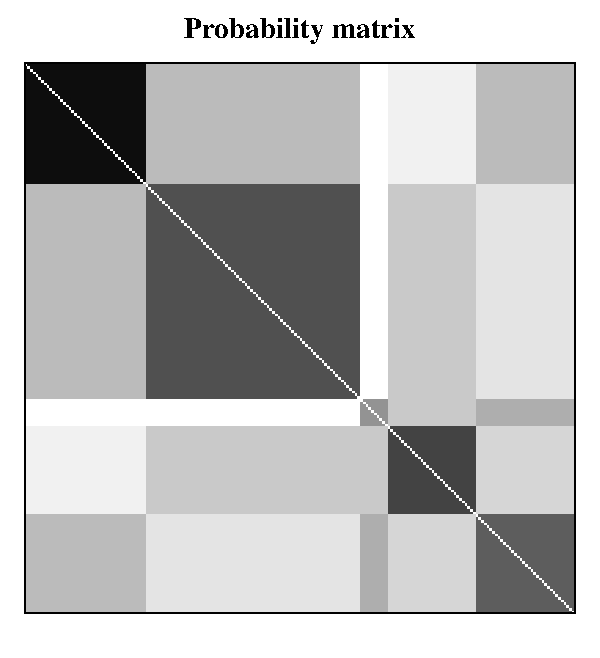
\includegraphics[height=\linewidth]{./Figures/SBM_P.pdf}
\end{subfigure}%
\begin{subfigure}{.45\textwidth}
  \centering
  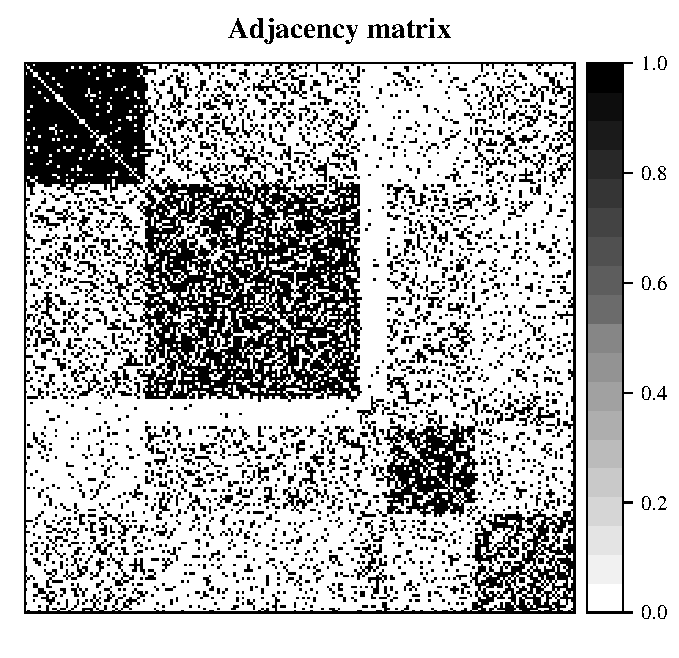
\includegraphics[height=\linewidth]{./Figures/SBM_A.pdf}
\end{subfigure}
\caption[Example illustrating the stochastic blockmodel]{Example illustrating the stochastic blockmodel. The parameters are given in Example~\ref{example:SBM}.
The left figure shows the probability matrix $P$ with $K = 5$ blocks and $n=200$ vertices and the right figure shows an adjacency matrix $A$ sampled under $\mathrm{SBM}(P)$.
While $A$ is a noisy version of $P$, much of the structure of $P$ is preserved in $A$, a property we will exploit in our estimation procedure.}
\label{fig:SBM_example}
\end{figure}

As discussed in Section~\ref{sec:RDPG}, the probability matrix $P$ in an RDPG is positive semidefinite. And now we argue that an SBM with a positive semidefinite $B$ can always be parameterized as an RDPG.
Firstly due to the positive semidefiniteness of $B$, we can decompose $B = \nu \nu^{\top}$ where $\nu \in \mathbb{R}^{K \times d}$. Define $\nu_1, \dots, \nu_K$ such that the rows of $\nu$ are given by $\nu_1^{\top}, \dots, \nu_K^{\top}$. Then $\nu_k$ can be regarded as the shared latent position for all vertices assigned to block $k$. Define $X = [X_1, \dots, X_n]^{\top} = [\nu_{\tau_1}, \dots, \nu_{\tau_n}]^{\top} \in \mathbb{R}^{n \times d}$. Then the SBM now can be parameterized as an RDPG since
\[
	\mathbb{P}(A_{ij} = 1) = B_{\tau_i, \tau_j} = \nu_{\tau_i}^{\top} \nu_{\tau_j}^{\phantom{\top}} = X_i^{\top} X_j \in [0, 1].
\]


\begin{definition} [SBM as RDPG]
\label{def:SBM_RDPG}
Consider an $\mathrm{RDPG}(\mathcal{X}, F)$ where $F$ is a distribution on $K$ point masses $\nu_1, \dots, \nu_K \in \mathcal{X}$ such that $\mathbb{P}(X_i = \nu_k) = \rho_k$ for $i \in [n]$ and $k \in [K]$, where the block proportion vector $\rho \in (0,1)^K$ with $\sum_{k=1}^K \rho_k = 1$. Then we denote this model by $\mathrm{SBM}(\rho, B)$ where $B = \nu^{\top} \nu$ with $\nu = [\nu_1, \dots, \nu_K]^{\top}$. Similarly, we can define $\tau \in [K]^n$ such that $X_i = \nu_{\tau_i}$. 
\end{definition}

For notational convenience we will refer to the sub-model of SBM with positive semidefinite $B$ as {\em{SBM}}.
As shown above, the SBM can be regard as an RDPG where all vertices in the same block have identical latent positions. In this work, we will always analyze SBM in an RDPG setting.


\begin{remark}
\label{remark:other_models}
As we mentioned, under the SBM, all vertices in the same block have identical latent positions. Rather than allowing vertices differ from each other as RDPG, SBM presumes all nodes within the same block have the same expected degree. To better describe complex networks in some situations, a bunch of generalizations of the SBM have been explored in order to incorporate the local variation of vertices to the block structure. \citet{airoldi2008mixed} proposed mixed membership stochastic blockmodels, which associates each vertex with multiple blocks with a probability vector rather than a single block as SBM requires. Also, in order to model variation of the expected degrees of different vertices within the same block, \citet{karrer2011stochastic} proposed degree-corrected SBM, which assigns additional parameters to each vertex to adjust the expected degree relatively. All these generalizations are trying to drag SBM towards RDPG a little bit so that the model can capture variations among vertices while keeping the community structure.
\end{remark}




\section{Weighted Random Graph Models}
\label{sec:weighted_graphs}

In this section, we shift our focus to the case where graphs are weighted and generalize the three models introduced in Section~\ref{sec:unweighted_graphs} respectively, i.e. the weighted independent edge model (WIEM) in Section~\ref{sec:WIEM}, the weighted random dot product graph model (WRDPG) in Section~\ref{sec:WRDPG}, and the weighted stochastic blockmodel (WSBM) as a WRDPG in Section~\ref{sec:WSBM}.

As a reminder, for weighted graphs, each edge is assigned with a positive real-valued weight, i.e. $\mathcal{A} = \mathbb{R}^{n \times n}_{\ge 0}$. So the adjacency matrices are not binary any more.


\subsection{Weighted Independent Edge Model}
\label{sec:WIEM}

As introduced in Section~\ref{sec:IEM}, under $\mathrm{IEM}(P)$, for $i, j \in [n]$ and $i < j$, the edge weight $A_{ij}$ is drawn from a Bernoulli distribution with parameter $P_{ij}$ independent of all other edges.
We first extend IEM to weighted independent edge model (WIEM).

\begin{definition} [Weighted Independent Edge Model]
\label{def:WIEM}
Consider a one-parameter family of distributions $\mathcal{F} = \{ f_{\theta} : \theta \in \Theta \subset \mathbb{R} \}$. Let the graph parameters be a matrix $P \in \Theta^{n \times n} \subset \mathbb{R}^{n \times n}$.
Then under a {\em{weighted independent edge model} (WIEM)} with respect to $\mathcal{F}$, for $i, j \in [n]$ and $i < j$, the edge weight between vertex $i$ and vertex $j$ is drawn from $f_{P_{ij}}$ independent of all other edges.
\end{definition}

Thus IEM is a special case of WIEM, with $\mathcal{F}$ representing the collection of Bernoulli distributions and $\Theta = [0, 1]$.

Note that the graphs considered in this paper are undirected without self-loops, and the parameter matrix $P$ can be considered to be symmetric and hollow. That is, for convenience, we still define the parameters to be an $n$-by-$n$ matrix while only $n \choose 2$ of them are active.



\subsection{Weighted Random Dot Product Graph}
\label{sec:WRDPG}

As discussed in Section~\ref{sec:RDPG}, the connectivity between two vertices in a graph generally depends on some hidden properties of the corresponding vertices. Such property is well captured by LPM as well as RDPG, which is a special case of LPM. In this section, we generalize RDPG to a weighted version so that it can model weighted graphs. 

\begin{definition}[Weighted Random Dot Product Graph]
Consider a collection of one-parameter distributions $\mathcal{F} = \{ f_{\theta}, \theta \in \Theta \subset \mathbb{R} \}$. The {\em{weighted random dot product graph (WRDPG)}} with respect to $\mathcal{F}$ is defined via consideration of latent position matrix $X \in \mathbb{R}^{n \times d}$ such that $X = [X_1, X_2, \dotsc, X_n]^{\top}$, where $X_i \in \mathbb{R}^d$ for all $i \in [n]$. The matrix $X$ is random and satisfies $\mathbb{P}\left[ X_i^{\top} X_j \in \Theta \right] = 1$ for all $i, j \in [n]$. Conditioned on $X$, the entries of the adjacency matrix $A$ are independent and $A_{ij}$ is a random variable following distribution $f_{\theta} \in \mathcal{F}$ with parameter $\theta = X_i^{\top} X_j $ for all $i < j \in [n]$.
\end{definition}

Under the WRDPG defined above, the parameter matrix $P = X X^{\top} \in \Theta^{n \times n} \subset \mathbb{R}^{n \times n}$ is automatically symmetric because the link function is the inner product. Moreover, to have symmetric graphs without self-loops, only $A_{ij}$ ($i < j$) are sampled while leaving the diagonals of $A$ to be all zeros.

After such extension, WRDPG inherits some properties from RDPG naturally, for example the positive defininteness of $P$, non-identifiability, etc. And similarly, since $P$ is still the outer product of the latent positions $X$ in WRDPG, it also motivates the low-rank estimator based on spectral decomposition for weighted graphs which will be discussed in later sections.




\subsection{Weighted Stochastic Blockmodel}
\label{sec:WSBM}

\begin{definition} [Weighted Stochastic Blockmodel]
\label{def:SBM}
Consider a collection of one-parameter distributions $\mathcal{F} = \{ f_{\theta}, \theta \in \Theta \subset \mathbb{R} \}$. A $K$-block {\em{weighted stochastic blockmodel (WSBM)}} with respect to $\mathcal{F}$ is defined as follows: Let block probability matrix be $B \in \Theta^{K \times K}$, and let the vector of block memberships be $\tau \in [K]^n$, where for each $i \in [n]$, $\tau_i = k$ means vertex $i$ is a member of block $k$. Then $A_{ij}$ follows distribution $f_{\theta} \in \mathcal{F}$ with parameter $\theta = B_{ij}$ independent of others for $i, j \in [n]$ and $i < j$.
\end{definition}

WSBM can be defined in a similar way in the scenario when the block probability matrix $B$ and block membership vector $\tau$ are random. As mentioned in Section~\ref{sec:SBM}, all analysis for unweighted graphs is based on RDPG setting. Likewise, in this section we will represent WSBM as WRDPG. Because of the structure of WRDPG, in order to consider WSBM as a WRDPG, the block probability matrix $B$ is assumed be positive semidefinite. From now on, we will denote the sub-model of WSBM with positive semi-definite $B$ as the WSBM.

\begin{definition} [WSBM as WRDPG]
\label{def:SBM_RDPG}
Consider a WRDPG with respect to $\mathcal{F}$ where each latent position $X_i$ can take one of the $K$ possible values $\nu_1, \dots, \nu_K$ such that $\mathbb{P}(X_i = \nu_k) = \rho_k$ for $i \in [n]$ and $k \in [K]$, where the block proportion vector $\rho \in (0,1)^K$ with $\sum_{k=1}^K \rho_k = 1$. Then this is a WSBM with respect to $\mathcal{F}$ where $B = \nu^{\top} \nu$ with $\nu = [\nu_1, \dots, \nu_K]^{\top}$. Similarly, we can define $\tau \in [K]^n$ such that $X_i = \nu_{\tau_i}$. 
\end{definition}

As shown above, the WSBM can be regard as a WRDPG where all vertices in the same block have identical latent positions. In later sections when considering weighted graphs, we will always analyze WSBM in a WRDPG setting.

















